\documentclass[runningheads]{llncs}

% EMO 2027 working draft. Full papers: 15 pages including references.
% Official template: Springer LNCS.

\usepackage[T1]{fontenc}
\usepackage[utf8]{inputenc}
\usepackage{amsmath,amssymb,mathtools}
\usepackage{booktabs}
\usepackage{graphicx}
\usepackage{algorithm}
\usepackage{algpseudocode}
\usepackage{xcolor}
\usepackage{xurl}
\usepackage{microtype}

\newcommand{\IR}{\operatorname{IR2}}
\newcommand{\Rtwo}{\mathrm{R2}}
\newcommand{\DeltaP}{\Delta_p}
\newcommand{\todo}[1]{\textcolor{red!70!black}{\textbf{[TODO: #1]}}}
\newcommand{\R}{\mathbb{R}}
\newcommand{\W}{\mathcal{W}}
\newcommand{\cIR}{C_{\IR}}

\title{IR2-EMOA: Multiobjective Selection Based on the Integral R2 Indicator}
\titlerunning{IR2-EMOA}

\author{Michael T. M. Emmerich\inst{1} \and
Lennart Sch\"apermeier\inst{2} \and
Pascal Kerschke\inst{2}}
\authorrunning{M. T. M. Emmerich, L. Sch\"apermeier, and P. Kerschke}

\institute{Faculty of Information Technology, University of Jyv\"askyl\"a, Jyv\"askyl\"a, Finland
\and
TU Dresden, Dresden, Germany\\
\email{\{lennart.schaepermeier,pascal.kerschke\}@tu-dresden.de}}
% TODO(author): confirm Michael's final affiliation and all author e-mail addresses.

\begin{document}
\maketitle

\begin{abstract}
Indicator-based environmental selection is attractive because it reduces the quality of an approximation set to a scalar criterion that can be used directly in survival decisions. SMS-EMOA is a prominent steady-state example and removes the solution with the smallest hypervolume contribution from the worst nondominated front. Hypervolume, however, is defined relative to a dominated, or dystopian, reference point. In this paper we propose \emph{Integral R2 EMOA} (IR2-EMOA), a steady-state evolutionary multiobjective optimization algorithm that instead uses the exact Integral R2 indicator. Integral R2 integrates the lower envelope of weighted Tchebycheff losses over a continuous weight simplex and is naturally specified by an ideal or utopian point. Unlike the commonly used finite-weight approximation of R2, the integral formulation is Pareto compliant. We use IR2 contributions for environmental selection. The bi-objective contribution formula is taken from the R2 v2 work of Sch\"apermeier and Kerschke; for three objectives we use perspective mapping to a hypervolume-analogue box decomposition and dimension sweep. This three-dimensional contribution computation is a supporting contribution rather than the main contribution of the paper. The resulting algorithm retains the simple steady-state structure of SMS-EMOA while replacing a dystopian-reference-point indicator by an ideal-point-based indicator. The empirical study is restricted to two and three objectives and assesses approximation sets by Integral R2, hypervolume, and the standard averaged Hausdorff distance $\Delta_p$.
\keywords{Evolutionary multiobjective optimization \and indicator-based selection \and Integral R2 \and steady-state EMOA \and quality indicators}
\end{abstract}

\section{Introduction}
\label{sec:introduction}

Evolutionary multiobjective optimization aims to approximate a set of mutually nondominated trade-off solutions rather than a single optimum. This makes environmental selection intrinsically set based. Indicator-based evolutionary algorithms address this issue by quantifying the quality of a candidate approximation set with a scalar set indicator and using the change in this value as a survival criterion.

SMS-EMOA is one of the clearest realizations of this principle. It combines steady-state evolution and nondominated sorting with hypervolume-based environmental selection: after inserting one offspring, one solution is deleted, and hypervolume contribution is used to discriminate within the relevant nondominated front~\cite{BeumeNaujoksEmmerich2007}. Efficient low-dimensional algorithms make this strategy especially attractive for two and three objectives~\cite{EmmerichFonseca2011}.

The hypervolume indicator is measured relative to a dominated, or dystopian, reference point. The choice of this point can influence both the numerical value and the distribution preferred by hypervolume-based selection. In contrast, the R2 family is naturally formulated relative to an ideal or utopian point through weighted Tchebycheff scalarizations. Such information can be more natural to specify: in many applications, meaningful best attainable or target values are known objective-wise even when no natural sufficiently bad reference point is available~\cite{SchaepermeierKerschke2025,Emmerich2026Preference}.

The classical R2 indicator is normally approximated with a finite set of weight vectors. This discretization makes evaluation simple and enables preference articulation, but it is only weakly Pareto compliant: a beneficial nondominated solution may fail to improve the indicator when no sampled weight vector exposes it~\cite{BrockhoffWagnerTrautmann2012,TrautmannWagnerBrockhoff2013}. Recent work returned to the continuous definition and showed that integrating a uniform continuum of weighted Tchebycheff utilities yields a Pareto-compliant unary indicator, together with exact algorithms in two objectives~\cite{SchaepermeierKerschke2025,JaszkiewiczZielniewicz2025}. Perspective mapping and box decomposition extend exact computation to three objectives in $O(n\log n)$ time and connect Integral R2 geometry to low-dimensional hypervolume algorithms without making Integral R2 itself a hypervolume indicator~\cite{Emmerich2026Perspective}.

This paper asks a focused algorithmic question: \emph{what happens if the steady-state indicator-based selection principle of SMS-EMOA is retained, but hypervolume contribution is replaced by exact IR2 contribution?} The resulting method, called Integral R2 EMOA (IR2-EMOA), is intended for two- and three-objective optimization. Its design is deliberately kept close to SMS-EMOA: each iteration creates one offspring, forms a $\mu+1$ candidate population, and selects a $\mu$-element survivor subset by deleting one solution, with nondominated rank as the primary criterion and indicator contribution as the secondary criterion in the worst front.

Our contributions are:
\begin{enumerate}
    \item We introduce IR2-EMOA as the direct Integral-R2 analogue of the steady-state SMS-EMOA design. Environmental selection maps a $\mu+1$ candidate set back to $\mu$ survivors and differs from the SMS-EMOA comparator only in the contribution indicator used within the worst nondominated front.
    \item As a supporting computational contribution, we realize all IR2 contributions in three objectives using perspective mapping. The mapping converts the geometry to a hypervolume-analogue anchored-box decomposition and dimension sweep; the ordinary box volume is replaced by integration with the Jacobian weight induced by the perspective map. In two objectives we use the exact IR2 contribution method already established in the R2 v2 work of Sch\"apermeier and Kerschke~\cite{SchaepermeierKerschke2025}, and do not claim a new bi-objective contribution algorithm here.
    \item We provide a reproducible six-problem diagnostic and benchmark setup for ZDT1--3 and DTLZ1, DTLZ2, and DTLZ7, with approximation quality assessed by Integral R2, hypervolume, and $\Delta_p$.
\end{enumerate}

\section{Background}
\label{sec:background}

\subsection{Multiobjective minimization and set dominance}

Consider a minimization problem
\begin{equation}
    \min_{x\in\mathcal{X}} F(x)
    = \bigl(f_1(x),\ldots,f_m(x)\bigr),
    \qquad m\in\{2,3\}.
\end{equation}
For objective vectors $y,y'\in\R^m$, $y$ dominates $y'$ if $y_i\le y'_i$ for all $i$ and the inequality is strict in at least one objective. A finite set is nondominated if none of its members dominates another. We write $z^\star$ for an ideal reference point satisfying $z_i^\star\le y_i$ for the approximation points considered below; a strictly better utopian point gives strict inequalities. For notational convenience define nonnegative loss vectors
\begin{equation}
    p=y-z^\star\in\R^m_{\ge0}.
\end{equation}
The derivations based on perspective mapping are stated first for strictly positive losses. Boundary cases with $p_i=0$, which occur when a point attains the ideal value in one objective, are handled by the continuous extension specified in Sect.~\ref{subsec:3d}; they must not be discarded as invalid points.

\subsection{Integral R2}
\label{subsec:ir2}

Let
\begin{equation}
    \mathcal{W}_{m-1}
    =\left\{w\in\R_{\ge0}^{m}:\sum_{i=1}^{m}w_i=1\right\}
\end{equation}
be the weight simplex and let $\nu$ denote the normalized uniform measure on it. For a loss vector $p$, the weighted Tchebycheff loss is
\begin{equation}
    \tau_w(p)=\max_{i=1,\ldots,m} w_i p_i.
\end{equation}
For a nonempty finite set $P$ of loss vectors, the Integral R2 indicator used in this paper is
\begin{equation}
\label{eq:ir2}
    \IR(P)
    =\int_{\mathcal{W}_{m-1}}
      \min_{p\in P}\tau_w(p)\,\mathrm{d}\nu(w).
\end{equation}
Thus smaller values are better. In two objectives, $w=(\lambda,1-\lambda)$ and~\eqref{eq:ir2} becomes
\begin{equation}
\label{eq:ir2-2d}
    \IR(P)=\int_0^1
    \min_{p\in P}
    \max\{\lambda p_1,(1-\lambda)p_2\}\,\mathrm{d}\lambda.
\end{equation}

The finite-weight R2 approximation replaces the integral by an average over a finite set $W$,
\begin{equation}
\label{eq:finite-r2}
    \Rtwo_W(P)=\frac{1}{|W|}\sum_{w\in W}\min_{p\in P}\tau_w(p).
\end{equation}
This discretization can leave nondominated points unseen by all sampled weights and is therefore only weakly Pareto compliant. With the continuous uniform weight distribution, Integral R2 is Pareto compliant~\cite{SchaepermeierKerschke2025,JaszkiewiczZielniewicz2025}.

This distinction matters for environmental selection. If $P$ dominates $Q$ and not conversely, Pareto compliance implies $\IR(P)<\IR(Q)$. Accordingly, a genuinely beneficial nondominated point produces a strict decrease of the indicator under nondegenerate conditions.

\subsection{SMS-EMOA and finite-weight R2-EMOA}

SMS-EMOA is a steady-state algorithm in which one offspring is generated and inserted at a time. Environmental selection applies nondominated sorting and removes one solution. Hypervolume contribution is used as the set-based secondary criterion in the relevant nondominated front~\cite{BeumeNaujoksEmmerich2007}. The method therefore provides the architectural template for IR2-EMOA, but the two methods encode different reference information: SMS-EMOA uses a dystopian reference point, while IR2-EMOA uses an ideal/utopian point.

Trautmann, Wagner, and Brockhoff introduced R2-EMOA, which uses contribution to a unary, finite-weight R2 indicator as a secondary selection criterion~\cite{TrautmannWagnerBrockhoff2013}. It is the most important R2-based comparator for the present study because it isolates the distinction between a finite weight set and continuous integration. R2-IBEA follows a different design: it removes dominance ranking and uses a binary R2 indicator inside an IBEA-style fitness assignment~\cite{PhanSuzuki2013}. We therefore treat R2-IBEA as related work rather than as the main architectural comparator.

\section{IR2 Contributions}
\label{sec:contributions}

Because Integral R2 is minimized, we define the IR2 contribution of a point as the positive increase of Integral R2 caused by deleting that point. This is the natural analogue of a hypervolume contribution for an indicator that is minimized.

\begin{definition}[IR2 contribution]
Let $P$ be a finite nondominated set with $|P|\ge2$ and $p\in P$. The IR2 contribution of $p$ is
\begin{equation}
\label{eq:deletion-loss}
    \cIR(p\mid P)
    =\IR(P\setminus\{p\})-\IR(P).
\end{equation}
\end{definition}

By monotonicity, $\cIR(p\mid P)\ge0$. If deleting $p$ makes the set strictly worse in the set-dominance sense, Pareto compliance gives $\cIR(p\mid P)>0$. Duplicates and points redundant under the adopted dominance convention can have zero IR2 contribution and should be removed before contribution computation.

The environmental selection rule of IR2-EMOA is therefore
\begin{equation}
\label{eq:least-ir2}
    p^-\in\arg\min_{p\in P}\cIR(p\mid P).
\end{equation}
Ties are broken uniformly at random unless stated otherwise.

\subsection{Two objectives}
\label{subsec:2d}

Exact bi-objective IR2 contributions are not derived again here. Sch\"apermeier and Kerschke already defined and computed the required least-contributor quantities in the R2 v2 work~\cite{SchaepermeierKerschke2025}. IR2-EMOA uses that contribution computation unchanged in two objectives. The new computational material below is therefore restricted to the three-objective case.

\subsection{Three objectives: perspective mapping and weighted exclusive boxes}
\label{subsec:3d}

For strictly positive $p\in\R^3_{>0}$ define its reciprocal corner in the usual way. For algorithmic use we extend the reciprocal map to nonnegative losses by
\begin{equation}
\label{eq:extended-reciprocal}
    b_i(p)=
    \begin{cases}
      1/p_i, & p_i>0,\\
      +\infty, & p_i=0.
    \end{cases}
\end{equation}
Thus, if a solution attains the ideal value in one objective, the corresponding reciprocal box is semi-infinite in that coordinate. This is the natural limiting convention $1/0:=+\infty$ and avoids perturbing extreme points away from the ideal boundary.

The perspective mapping developed in~\cite{Emmerich2026Perspective} transforms the subgraph of the lower Tchebycheff envelope into the complement of a union of anchored boxes in reciprocal objective space. It thereby permits a hypervolume-analogue box decomposition and dimension sweep. In three objectives, the absolute Jacobian determinant of the perspective map provides the weight
\begin{equation}
\label{eq:density}
    \omega(x)=\left|\det D\Psi(x)\right|
    =\frac{1}{(x_1+x_2+x_3)^4}.
\end{equation}
We refer to $\omega$ as the \emph{Jacobian weight}. Because~\eqref{eq:ir2} uses the normalized uniform measure on the two-dimensional simplex, the corresponding weighted volume is multiplied by $(3-1)!=2$. Computing the three-dimensional IR2 contributions in this way is a supporting contribution of the present paper, not its main algorithmic contribution.

For $|P|\ge2$, let $E_p$ be the region of the anchored reciprocal box of $b(p)$ that is not covered by the reciprocal boxes of any other point. Then the IR2 contribution is the weighted exclusive measure
\begin{equation}
\label{eq:weighted-exclusive}
    \cIR(p\mid P)=2\int_{E_p}\omega(x)\,\mathrm{d}x.
\end{equation}
This is the key bridge to low-dimensional contribution algorithms. The combinatorial decomposition into exclusive orthogonal boxes is independent of the measure used inside each box. Hence a contribution sweep that emits disjoint exclusive boxes can be reused by replacing ordinary volume with a weighted box primitive.

The weighted box primitive needs one boundary convention that ordinary hypervolume volume computations can ignore. Let
\[
    Q=\prod_{j=1}^{3}[\ell_j,u_j],
    \qquad 0\le \ell_j\le u_j\le +\infty.
\]
A hypervolume-contribution decomposition may emit a degenerate box because two event coordinates coincide. Such a box has zero three-dimensional measure even if one of its corners is the singular origin. We therefore define the degenerate case \emph{before} evaluating the eight corner terms:
\begin{equation}
\label{eq:weighted-box}
\mu(Q)=
\begin{cases}
0,
& \text{if }u_j=\ell_j\text{ for at least one }j,\\[1mm]
\displaystyle
\sum_{\epsilon\in\{0,1\}^3}
(-1)^{3-|\epsilon|}\,\Phi\!\left(c(\epsilon)\right),
& \text{otherwise},
\end{cases}
\end{equation}
where $c_j(0)=\ell_j$, $c_j(1)=u_j$, and
\begin{equation}
\label{eq:weighted-box-node}
\Phi(x_1,x_2,x_3)=
\begin{cases}
0, & \text{if at least one }x_j=+\infty,\\[1mm]
-\dfrac{1}{6(x_1+x_2+x_3)},
& \text{if }x_1+x_2+x_3>0.
\end{cases}
\end{equation}
For a nondegenerate box with $\ell_1=\ell_2=\ell_3=0$ the weighted integral is divergent; such a positive-volume box contains the singular origin and is not a valid exclusive contribution box. In contrast, a zero-width box touching the origin has value exactly zero by the first line of~\eqref{eq:weighted-box}. This ordering of the cases is essential: applying the eight-corner formula first would create a spurious undefined $\infty-\infty$ cancellation for geometrically null boxes.

Equations~\eqref{eq:weighted-box}--\eqref{eq:weighted-box-node} also cover an objective value equal to the ideal point through~\eqref{eq:extended-reciprocal}: the corresponding reciprocal upper bound is $+\infty$, and every corner term involving that upper bound contributes zero. Hence repeated contribution-sweep coordinates, zero-width slabs, and ideal-point boundary coordinates require no numerical perturbation. Every nondegenerate emitted box is still integrated in constant time with at most eight node evaluations.

The all-contributions algorithm of Emmerich and Fonseca computes all three-dimensional hypervolume contributions in $O(n\log n)$ time and $O(n)$ space~\cite{EmmerichFonseca2011}. The perspective result implies that its exclusive-region decomposition can be transported to Integral R2 by weighting the emitted boxes~\cite{Emmerich2026Perspective}. Our implementation follows the same sweep organization in reciprocal space and uses coordinate compression together with array-based predecessor/successor information; a Fenwick tree is used for active-rank queries, while path-compressed skip pointers avoid repeated traversal of deleted skyline nodes. The geometric ordering is unchanged; only the box accumulator is replaced by $2\mu(Q)$.

\begin{algorithm}[t]
\caption{Three-objective all-contribution framework}
\label{alg:all3d}
\begin{algorithmic}[1]
\Require Nondominated loss vectors $P\subset\R^3_{\ge0}$
\Ensure $\cIR(p\mid P)$ for all $p\in P$
\State map every $p$ to $b(p)$ using Eq.~\eqref{eq:extended-reciprocal}
\State coordinate-compress the sweep coordinates
\State initialize contribution accumulator $C[p]\gets0$ for all $p$
\State initialize Fenwick/pointer skyline structure
\For{each sweep event in the third coordinate}
    \State update the active two-dimensional skyline
    \State emit every newly determined disjoint exclusive box $Q$ with owner $p$
    \If{$Q$ is degenerate in at least one coordinate}
        \State skip $Q$ (its weighted measure is exactly zero)
    \Else
        \State $C[p]\gets C[p]+2\mu(Q)$ using Eqs.~\eqref{eq:weighted-box}--\eqref{eq:weighted-box-node}
    \EndIf
\EndFor
\State \Return $C$
\end{algorithmic}
\end{algorithm}

\paragraph{Complexity.}
The target implementation preserves the $O(n\log n)$ sorting/sweep bound and $O(n)$ storage of the low-dimensional contribution decomposition, because each emitted orthogonal box is replaced by a constant-time weighted-box evaluation. Degenerate boxes are rejected in $O(1)$ time before the eight-node evaluation, exactly as zero-volume slabs are discarded by the box emitter; this does not change the asymptotic bound. \todo{In the final version, include the complete ownership invariant and a self-contained proof that the chosen Fenwick/pointer implementation emits exactly the same exclusive boxes as the underlying three-dimensional all-contributions sweep.}

\section{Integral R2 EMOA}
\label{sec:emoa}

IR2-EMOA deliberately mirrors the steady-state structure of SMS-EMOA. Let $\mu$ be the population size. One offspring is created, evaluated, and inserted, producing a $\mu+1$ candidate set. Environmental selection then chooses a $\mu$-element survivor subset by deleting exactly one solution. Nondominated sorting identifies the worst front from which this deletion must occur. If the worst front contains more than one point, exact IR2 contributions are calculated within that front and the point with the smallest IR2 contribution is discarded.

The restriction to the worst front is inherited from the SMS-EMOA design principle: Pareto rank remains the primary criterion, while the indicator is used only to discriminate among solutions of equal rank. This avoids allowing an indicator value to preserve a dominated point at the expense of a nondominated one. Thus the proposed algorithm changes the set indicator used by SMS-EMOA while intentionally leaving the $\mu+1\rightarrow\mu$ steady-state architecture unchanged.

\paragraph{Remark on $\mu+\lambda$ survivor selection.}
A natural generational extension would create $\lambda>1$ offspring and then select an indicator-optimal $\mu$-subset from a $\mu+\lambda$ equal-rank candidate set. For Integral R2 this is a substantially harder optimization problem than the single-deletion step used here. In two objectives, exact fixed-cardinality Integral R2 subset selection can be realized efficiently by dynamic programming and Monge structure~\cite{Emmerich2026Subset2D}. In three objectives, however, exact fixed-cardinality Integral R2 subset selection is NP-hard~\cite{Emmerich2026Subset3D}. This complexity separation is an additional reason to retain the SMS-EMOA-style steady-state $\mu+1\rightarrow\mu$ design in the present three-objective algorithm.

\begin{algorithm}[t]
\caption{Integral R2 EMOA (IR2-EMOA)}
\label{alg:ir2emoa}
\begin{algorithmic}[1]
\Require Population size $\mu$, evaluation budget $B$, ideal point $z^\star$
\State initialize and evaluate population $P$ with $|P|=\mu$
\While{number of evaluations $<B$}
    \State select two parents by binary tournament
    \State create one offspring $x$ using SBX crossover and polynomial mutation
    \State evaluate $x$ and set $Q\gets P\cup\{x\}$
    \State nondominated-sort $Q$ into $F_1,\ldots,F_k$
    \State $F\gets F_k$ \Comment{worst front}
    \If{$|F|=1$}
        \State remove the unique member of $F$
    \Else
        \State compute $\cIR(y-z^\star\mid F-z^\star)$ for every $y\in F$
        \State remove one $y^-\in\arg\min_{y\in F}\cIR(y-z^\star\mid F-z^\star)$
    \EndIf
    \State $P\gets Q\setminus\{y^-\}$
\EndWhile
\State \Return the nondominated subset of $P$
\end{algorithmic}
\end{algorithm}

No additional diversity operator, decomposition mechanism, or adaptive weight-vector scheme is introduced. For real-valued DTLZ problems, we use simulated binary crossover and polynomial mutation with the same settings for all compared algorithms. Parent selection is a standard binary tournament. This intentionally keeps the experimental question centered on environmental selection rather than variation-operator tuning.

\subsection{Reference information}

The most visible conceptual difference from SMS-EMOA is the direction of reference information. Hypervolume needs a dystopian point that is componentwise worse than the region intended to contribute. Integral R2 instead measures weighted loss from an ideal/utopian point. We do not claim that an ideal point is universally easier to specify, but it can be more natural in problems where objective-wise best values or meaningful targets are known while no principled upper bound is available. The experiments therefore use problem-defined ideal points and do not tune them per algorithm run.

\section{Experimental Design}
\label{sec:experiments}

The study is intentionally restricted to the questions needed to evaluate IR2-EMOA within a 15-page conference paper.

\subsection{Algorithms}

The main comparison contains three methods:
\begin{enumerate}
    \item \textbf{IR2-EMOA}: the proposed steady-state algorithm with exact IR2 contributions;
    \item \textbf{SMS-EMOA}: the same steady-state indicator-selection paradigm using hypervolume contribution~\cite{BeumeNaujoksEmmerich2007};
    \item \textbf{R2-EMOA}: the finite-weight-vector R2 algorithm of Trautmann, Wagner, and Brockhoff~\cite{TrautmannWagnerBrockhoff2013}.
\end{enumerate}
All three algorithms use identical initialization, binary-tournament mating selection, simulated binary crossover, polynomial mutation, population size, and evaluation budget. For each problem/run pair they start from the same initial population and use the same variation random seed. Finite-weight R2-EMOA uses 101 uniformly spaced weights in two objectives and the 120-vector simplex lattice in three objectives. The SMS-EMOA branch is the exact steady-state analogue of IR2-EMOA: only the secondary contribution calculation is exchanged. Its hypervolume reference point is placed 10\% beyond the coordinatewise nadir of the current worst nondominated front relative to that front's coordinate range; equivalently, after affine front normalization, the reference point is $(1.1,\ldots,1.1)$.

R2-IBEA is discussed in related work but is not a main baseline because its binary-indicator fitness assignment removes dominance ranking and therefore tests a different algorithmic architecture~\cite{PhanSuzuki2013}.

\subsection{Benchmark problems}

The diagnostic and benchmark set contains six standard problems: ZDT1, ZDT2, and ZDT3 in two objectives, and DTLZ1, DTLZ2, and DTLZ7 in three objectives~\cite{DebThieleLaumannsZitzler2002}. To keep this first controlled benchmark inexpensive, the decision-space dimension is fixed to five for all six problems. This leaves the analytical Pareto fronts unchanged while reducing the number of distance variables in the search. Each run uses a population of $50$ and a budget of $10{,}000$ function evaluations. For performance assessment, each known Pareto front is represented by a deterministic reference set of $10{,}000$ points. The same reference sets are used by all methods and by all three reported performance indicators.

\subsection{Performance measures}

Approximation quality is assessed by three complementary set indicators: Integral R2, hypervolume (HV), and the standard averaged Hausdorff distance $\Delta_p$~\cite{SchuetzeEtAl2012}. Integral R2 is evaluated exactly with the benchmark's componentwise ideal point. For performance assessment, HV uses one fixed reference point per problem, obtained by shifting the sampled Pareto-front nadir outward by 10\% of the ideal-to-nadir range; this assessment reference is identical for all algorithms and should not be confused with the adaptive front-wise reference used internally by SMS-EMOA selection. For $\Delta_p$, each problem uses the same deterministic $10{,}000$-point Pareto-front reference set. We use $p=2$ throughout.

The three indicators emphasize different distribution properties. Integral R2 measures quality with respect to the continuous family of weighted Tchebycheff scalarizations; HV measures dominated objective-space volume relative to a fixed dystopian point; and $\Delta_p$ jointly reflects convergence and coverage. Reporting all three prevents the empirical assessment from being tied exclusively to either the IR2 selection criterion or the hypervolume selection criterion.

The six-panel ZDT/DTLZ gallery below is retained as a diagnostic visualization rather than as a substitute for quantitative benchmarking. Its purpose is to make the distribution induced by IR2-based environmental selection directly visible, including behavior at extreme points and on disconnected fronts.

\subsection{Runtime experiment}

The indicator-selection machinery is evaluated separately from optimization quality. For random nondominated point sets of increasing size $n$, we measure wall-clock time for all IR2 contributions in two and three objectives. The optimized implementation is checked against the brute-force reference
\begin{equation}
    \cIR(p\mid P)=\IR(P\setminus\{p\})-\IR(P)
\end{equation}
computed independently for every $p$. Tests include random fronts, nearly tied coordinates, exact repeated event coordinates, zero-width emitted boxes, extreme points with one or more objective values equal to the ideal point, and duplicated input before filtering. Boundary tests verify explicitly that degenerate boxes return zero before any singular corner is evaluated and that reciprocal upper bounds $+\infty$ are handled by Eq.~\eqref{eq:weighted-box-node}. Fixed seeds and exact agreement up to a stated numerical tolerance are used for reproducibility.

\subsection{Statistical protocol}

We use ten paired runs per algorithm/problem combination. Within each problem and run index, all three algorithms share the same initial population and variation random seed. The exact variation seeds and the corresponding initialization seeds are stored explicitly in \texttt{seeds.csv}; the initialization seed is the variation seed plus 17. Table~\ref{tab:benchmark10} reports the median together with the sample standard deviation (median $\pm$ SD) computed from the ten run-wise values. Complete run-wise results are provided with the paper. The present ten-run experiment is intended as a controlled benchmark rather than a definitive large-scale statistical comparison, so we do not attach significance claims to small differences.

\section{Results}
\label{sec:results}

\subsection{Ten-run ZDT/DTLZ benchmark}

Table~\ref{tab:benchmark10} reports median performance and sample standard deviation over ten paired runs for each of the three environmental-selection mechanisms. Every run uses five decision variables, population size $50$, and $10{,}000$ function evaluations. The table deliberately reports all three assessment indicators: exact Integral R2, HV, and $\Delta_p$. The complete run-wise values and exact paired seeds are supplied with the code; the standard deviations make unusually variable cases immediately visible.

\begin{table}[t]
\centering
\caption{Ten-run benchmark results as median $\pm$ sample standard deviation with five decision variables, population size $50$, and $10{,}000$ evaluations. Smaller is better for IR2 and $\Delta_p$; larger is better for HV. Exact paired seeds and all run-wise values are provided in the repository.}
\label{tab:benchmark10}
\scriptsize
\setlength{\tabcolsep}{2.5pt}
\begin{tabular}{llccc}
\toprule
Problem & Algorithm & IR2 $\downarrow$ & HV $\uparrow$ & $\Delta_p\downarrow$\\
\midrule
ZDT1 & IR2-EMOA & $\mathbf{0.133342\pm4.22e-06}$ & $0.865733\pm0.000265$ & $0.011116\pm0.000522$\\
 & finite R2-EMOA & $0.133398\pm1.43e-05$ & $0.865033\pm0.000317$ & $0.012377\pm0.000617$\\
 & SMS-EMOA & $0.133517\pm2.56e-05$ & $\mathbf{0.867438\pm2.12e-05}$ & $\mathbf{0.008516\pm8.45e-05}$\\
\addlinespace[1pt]
ZDT2 & IR2-EMOA & $\mathbf{0.198800\pm3.49e-06}$ & $0.533803\pm0.000132$ & $0.014508\pm0.000656$\\
 & finite R2-EMOA & $0.198893\pm1.24e-05$ & $0.533085\pm0.000261$ & $0.015656\pm0.001247$\\
 & SMS-EMOA & $0.198820\pm8.92e-06$ & $\mathbf{0.534296\pm3.00e-05}$ & $\mathbf{0.011113\pm0.000343}$\\
\addlinespace[1pt]
ZDT3 & IR2-EMOA & $\mathbf{0.196016\pm0.013668}$ & $1.092857\pm0.009866$ & $0.015049\pm0.025889$\\
 & finite R2-EMOA & $0.196056\pm0.013672$ & $1.092395\pm0.009974$ & $0.016551\pm0.027011$\\
 & SMS-EMOA & $0.196108\pm1.87e-05$ & $\mathbf{1.094366\pm1.77e-05}$ & $\mathbf{0.012321\pm0.000426}$\\
\addlinespace[1pt]
DTLZ1 & IR2-EMOA & $\mathbf{0.033365\pm0.000179}$ & $0.133053\pm0.000623$ & $\mathbf{0.029741\pm0.000326}$\\
 & finite R2-EMOA & $0.034492\pm0.000679$ & $0.128569\pm0.000860$ & $0.085245\pm0.063017$\\
 & SMS-EMOA & $0.033834\pm0.000207$ & $\mathbf{0.137431\pm0.000233}$ & $0.031334\pm1.261365$\\
\addlinespace[1pt]
DTLZ2 & IR2-EMOA & $\mathbf{0.094891\pm6.70e-06}$ & $0.726085\pm0.000636$ & $0.090076\pm0.001392$\\
 & finite R2-EMOA & $0.095394\pm4.63e-05$ & $0.692045\pm0.001923$ & $\mathbf{0.083892\pm0.001283}$\\
 & SMS-EMOA & $0.094952\pm1.70e-05$ & $\mathbf{0.735302\pm0.000119}$ & $0.117048\pm0.001852$\\
\addlinespace[1pt]
DTLZ7 & IR2-EMOA & $0.458422\pm0.182414$ & $1.172993\pm0.106857$ & $0.520688\pm0.261109$\\
 & finite R2-EMOA & $\mathbf{0.229395\pm0.200067}$ & $1.129139\pm0.062432$ & $0.246245\pm0.267430$\\
 & SMS-EMOA & $0.233253\pm0.268388$ & $\mathbf{1.409654\pm0.211124}$ & $\mathbf{0.131598\pm0.428380}$\\
\bottomrule
\end{tabular}
\end{table}

The results should be read as a comparison of selection-induced distributions rather than as evidence for a universally best indicator. By the median, IR2-EMOA gives the smallest IR2 on five of the six problems; the exception is DTLZ7, where finite R2-EMOA has the smallest median IR2. SMS-EMOA gives the largest median HV on all six problems. The cross-indicator picture is more varied: SMS-EMOA gives the smallest median $\Delta_p$ on the three ZDT problems and DTLZ7, IR2-EMOA on DTLZ1, and finite R2-EMOA on DTLZ2. The comparatively large standard deviations on ZDT3, DTLZ1, and especially DTLZ7 reveal occasional poorly converged outlying runs that the medians deliberately downweight. DTLZ7 remains under-converged at the common $10{,}000$-evaluation budget for several runs; this is consistent with the diagnostic gallery, for which we deliberately used a larger $60{,}000$-evaluation budget on DTLZ7. The ten-run experiment is therefore descriptive, and all individual run values and seeds are retained in the repository.

\subsection{Single-shot gallery}

Figure~\ref{fig:single-shot-gallery} collects six exact-ideal single-shot plots as a diagnostic of the distribution properties induced by IR2-based selection.  The three ZDT cases are shown in two objectives, whereas DTLZ1, DTLZ2, and DTLZ7 are shown in three objectives.  All runs use a population size of $60$ and seed $2027$; the budget is $30{,}000$ evaluations except for DTLZ7, which uses $60{,}000$ evaluations.

\begin{figure}[t]
\centering
\setlength{\tabcolsep}{3pt}
\renewcommand{\arraystretch}{1.0}
\begin{tabular}{cc}
\textbf{ZDT1 (2D), 30k evals} & \textbf{ZDT2 (2D), 30k evals}\\[-1mm]
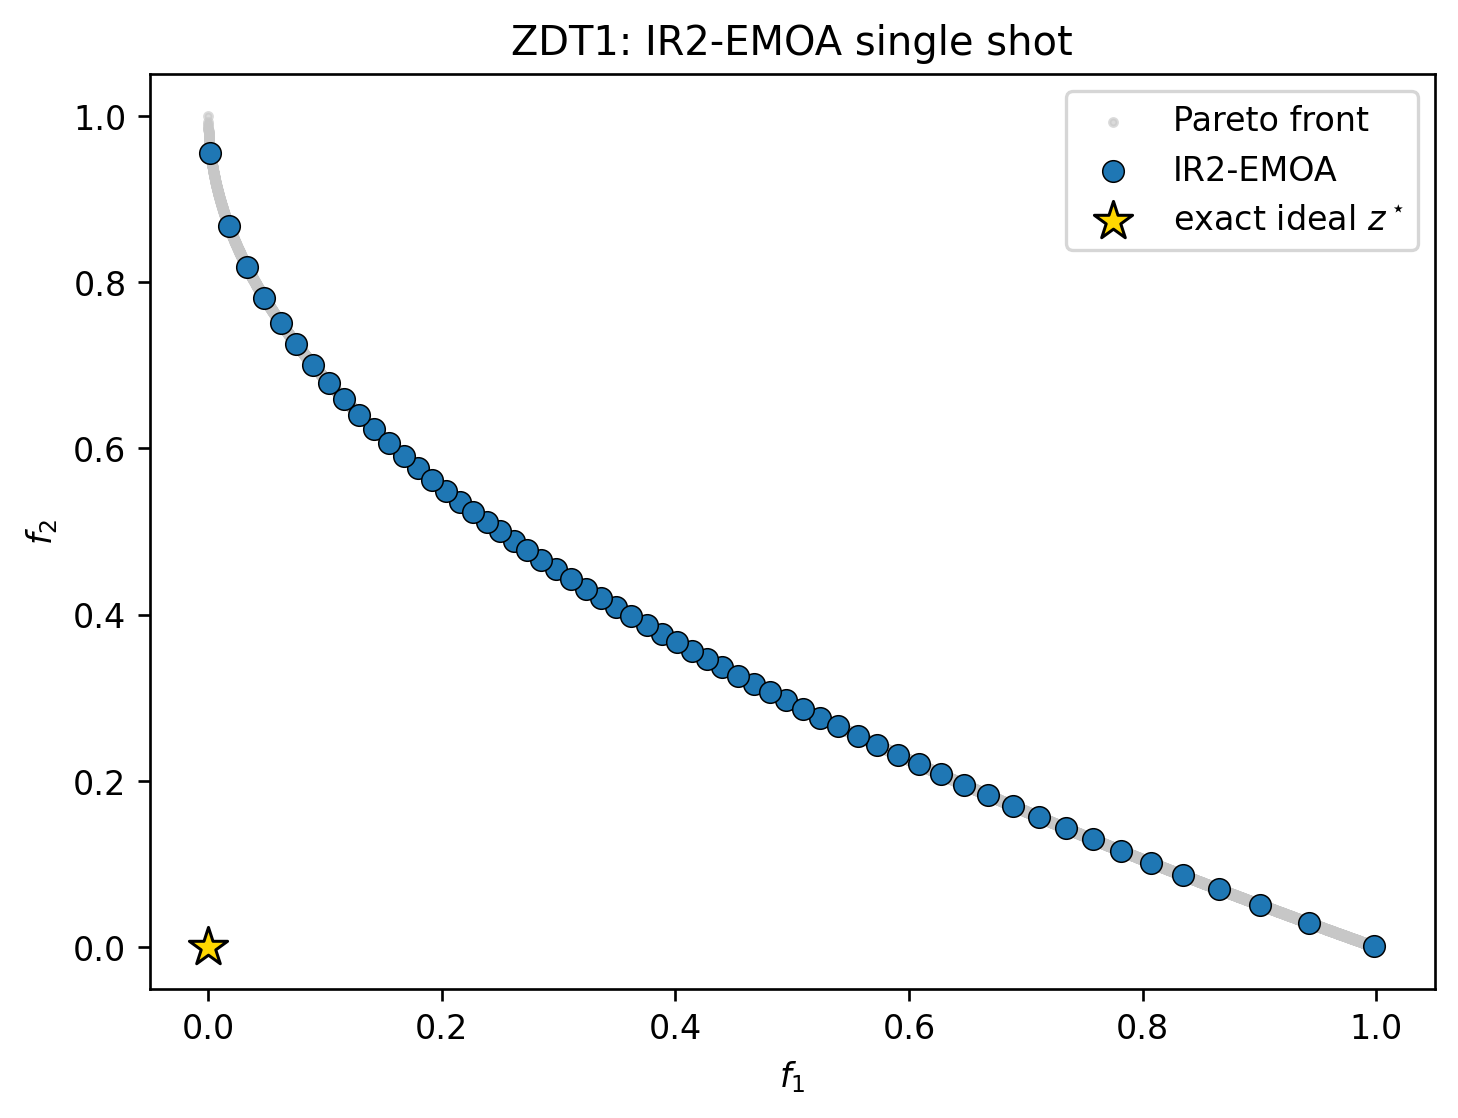
\includegraphics[width=0.45\linewidth]{single_shot_zdt1_2d_exact_ideal_30000evals.png} &
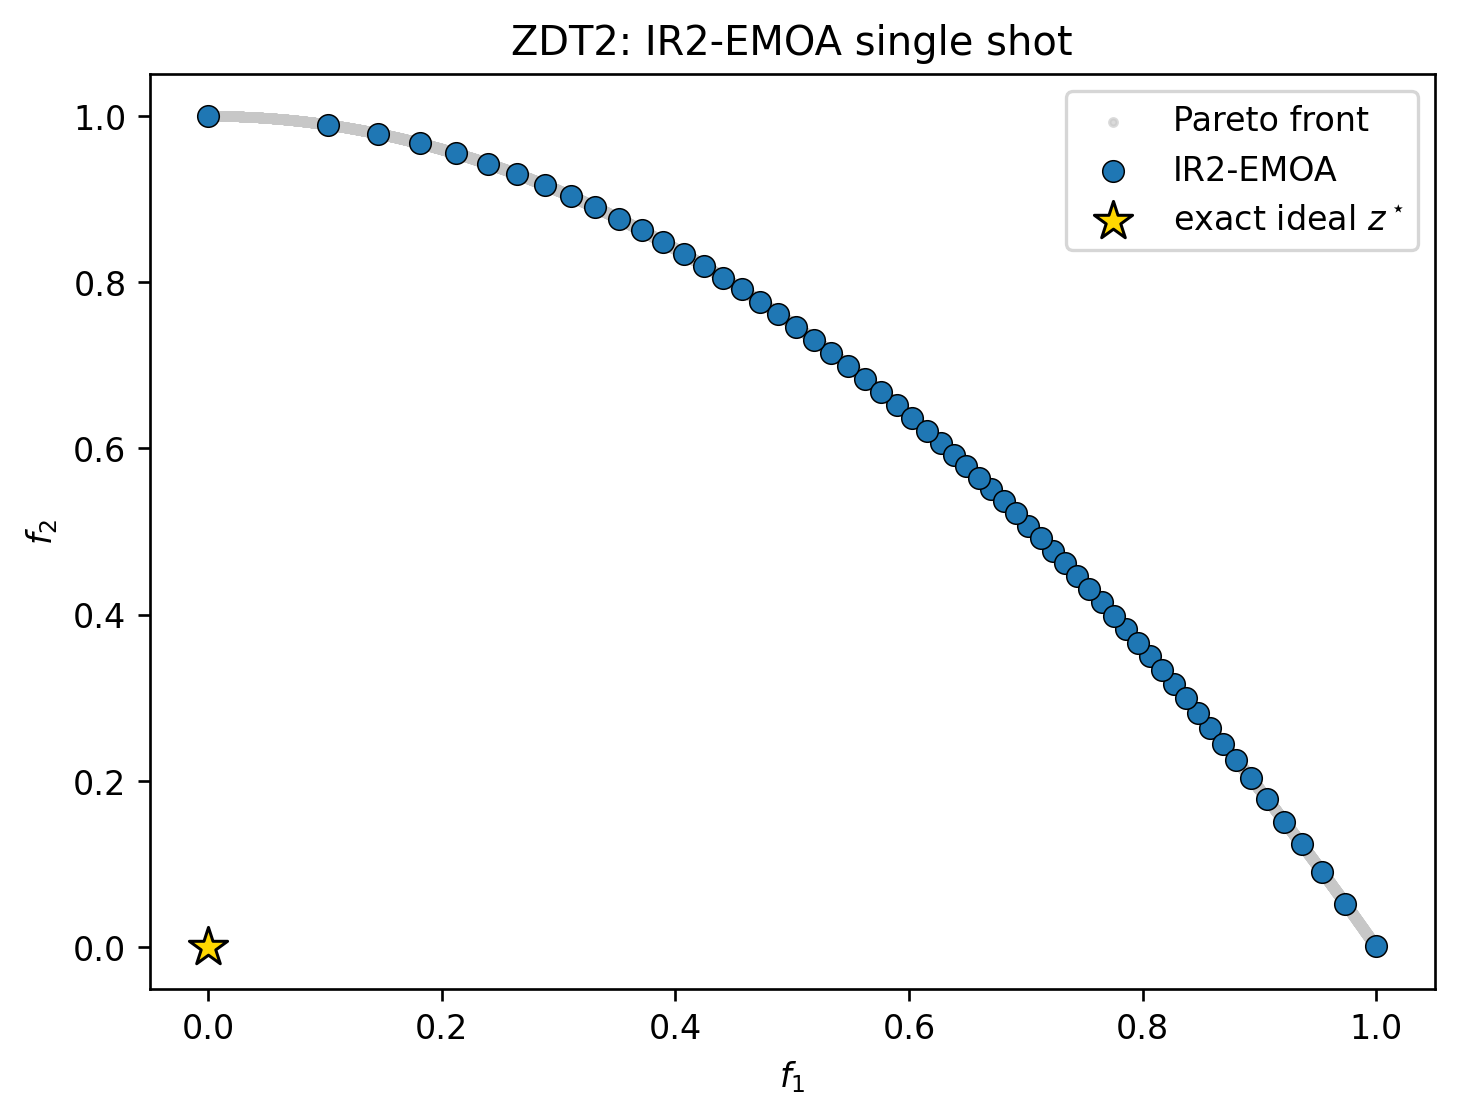
\includegraphics[width=0.45\linewidth]{single_shot_zdt2_2d_exact_ideal_30000evals.png}\\[1mm]
\textbf{ZDT3 (2D), 30k evals} & \textbf{DTLZ1 (3D), 30k evals}\\[-1mm]
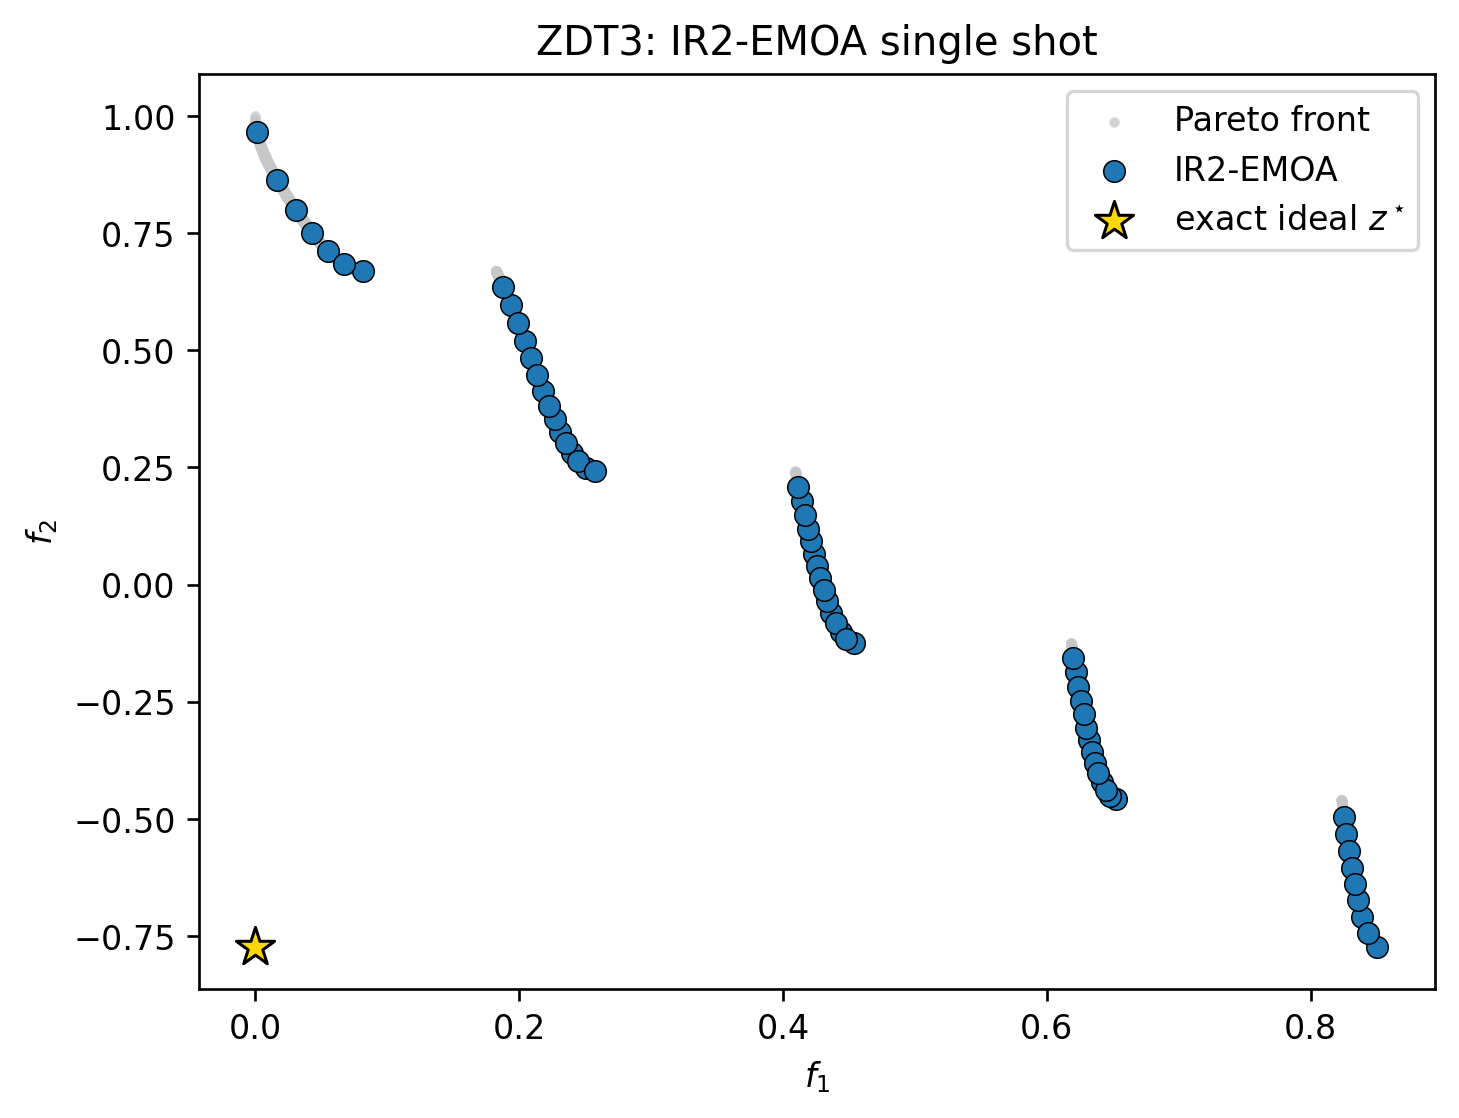
\includegraphics[width=0.45\linewidth]{single_shot_zdt3_2d_exact_ideal_30000evals.png} &
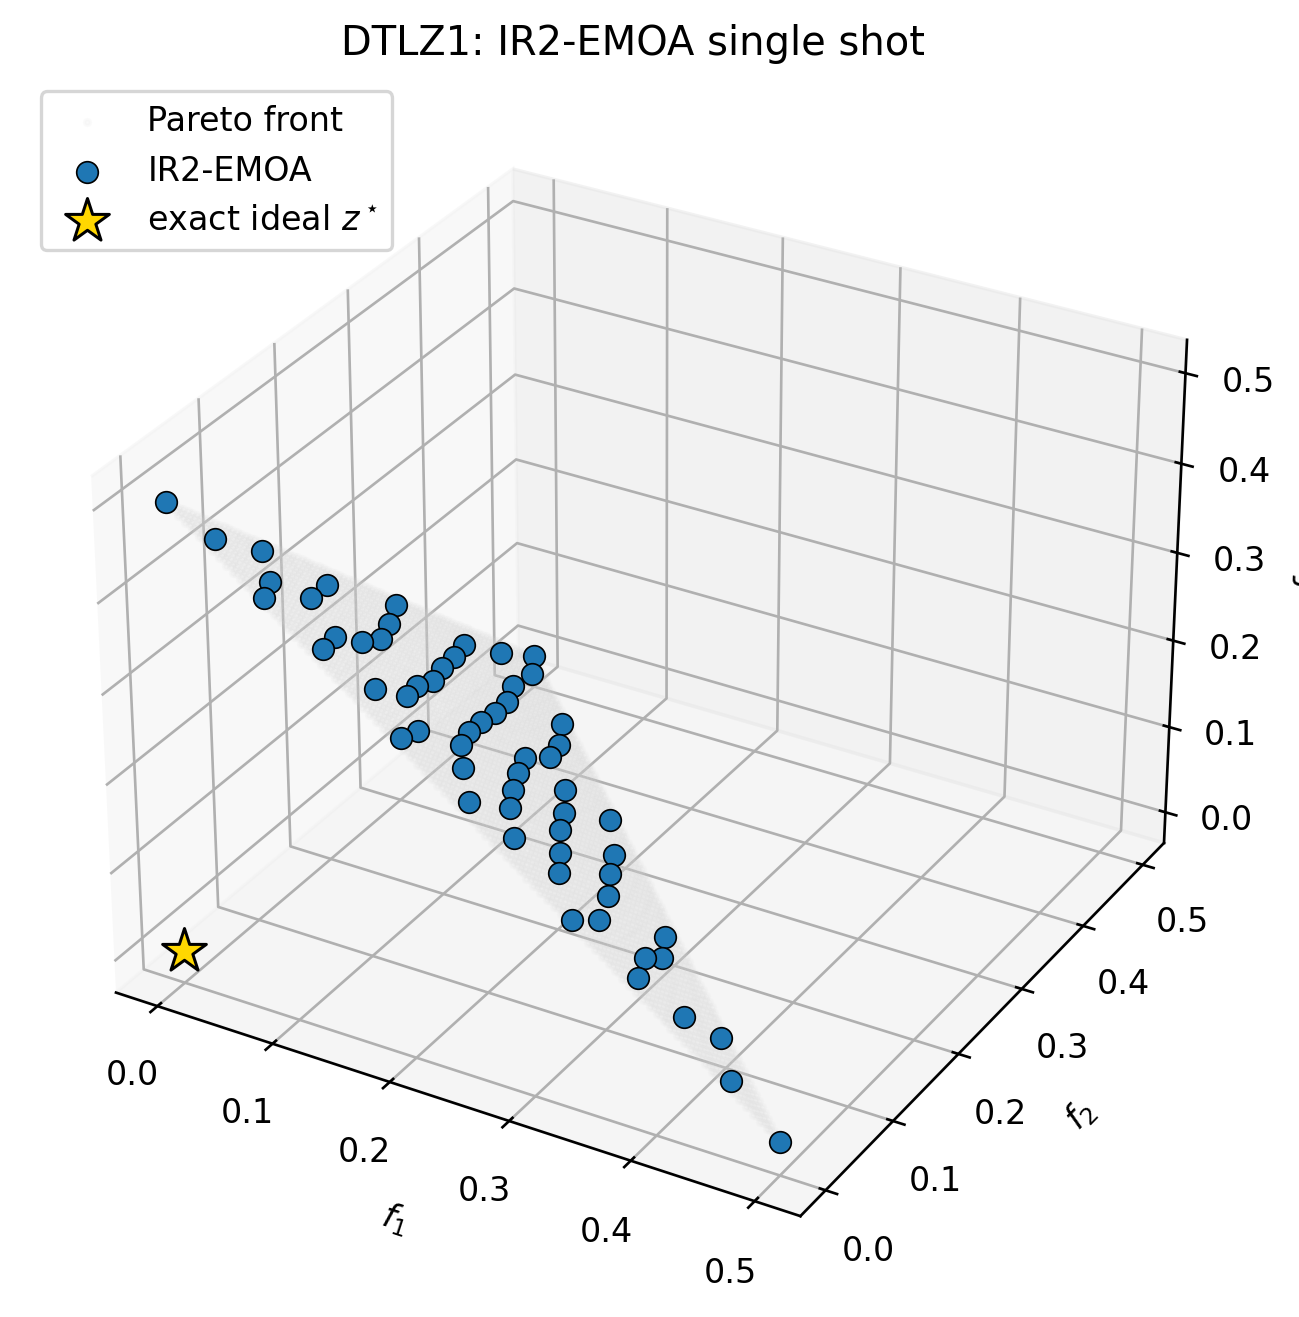
\includegraphics[width=0.45\linewidth]{single_shot_dtlz1_3d_exact_ideal_30000evals.png}\\[1mm]
\textbf{DTLZ2 (3D), 30k evals} & \textbf{DTLZ7 (3D), 60k evals}\\[-1mm]
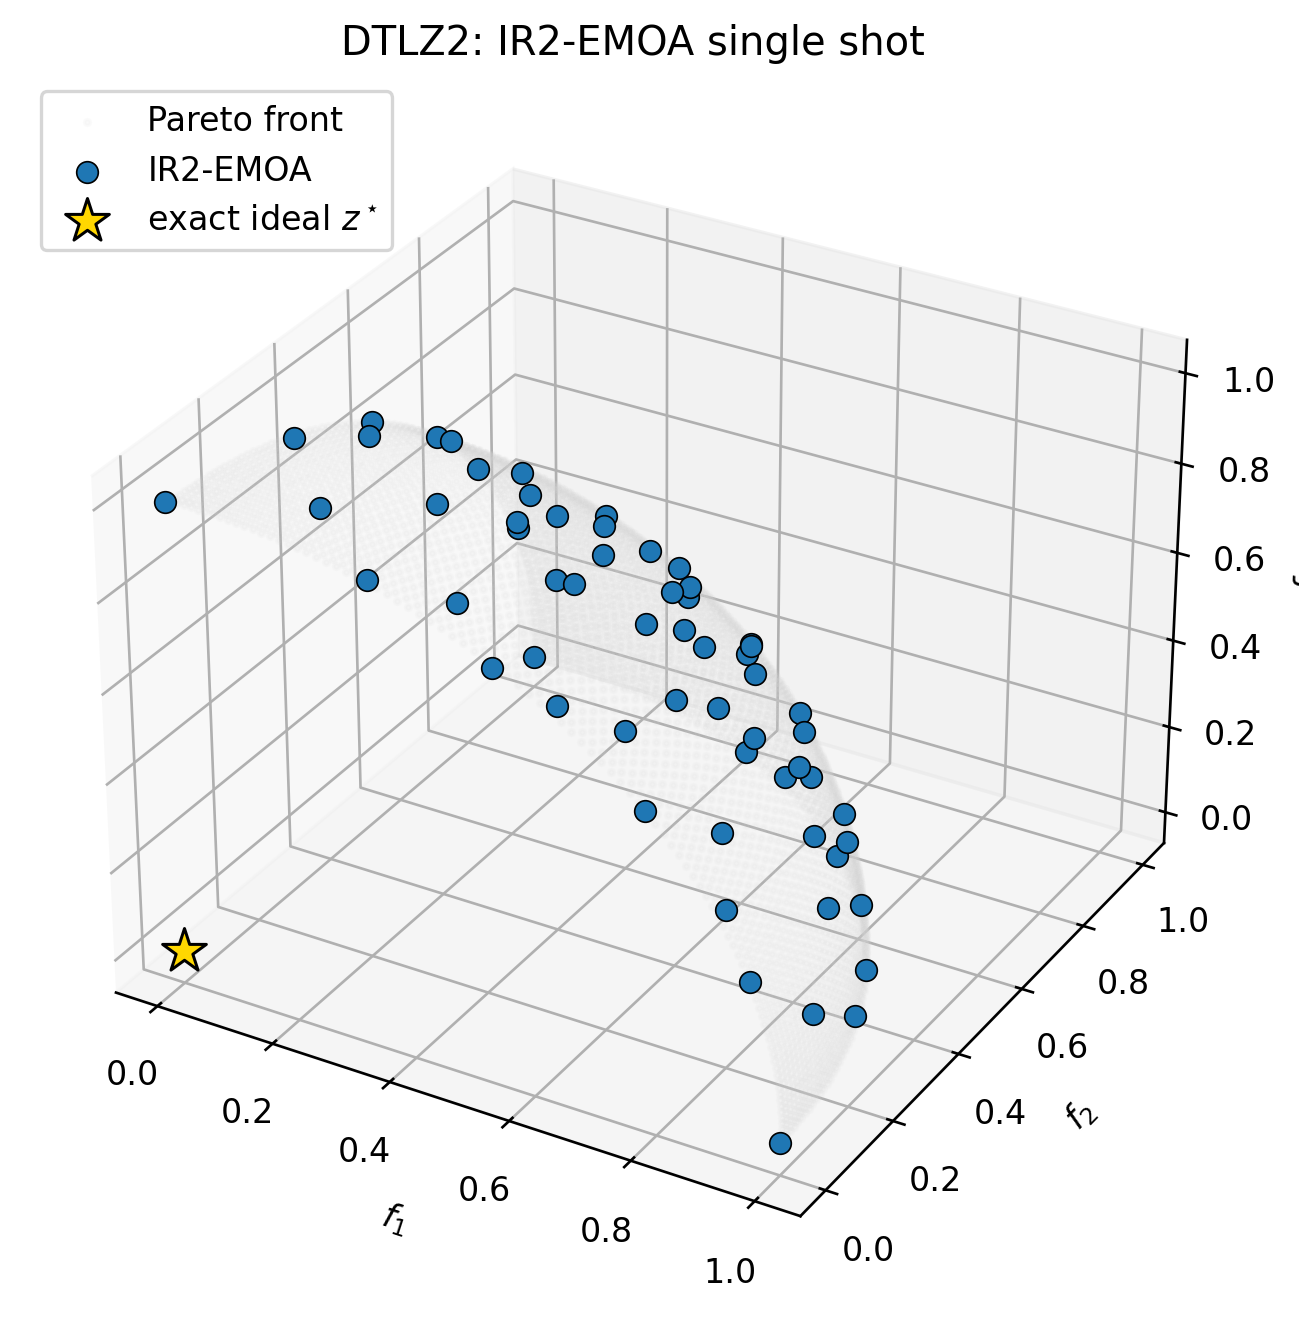
\includegraphics[width=0.45\linewidth]{single_shot_dtlz2_3d_exact_ideal_30000evals.png} &
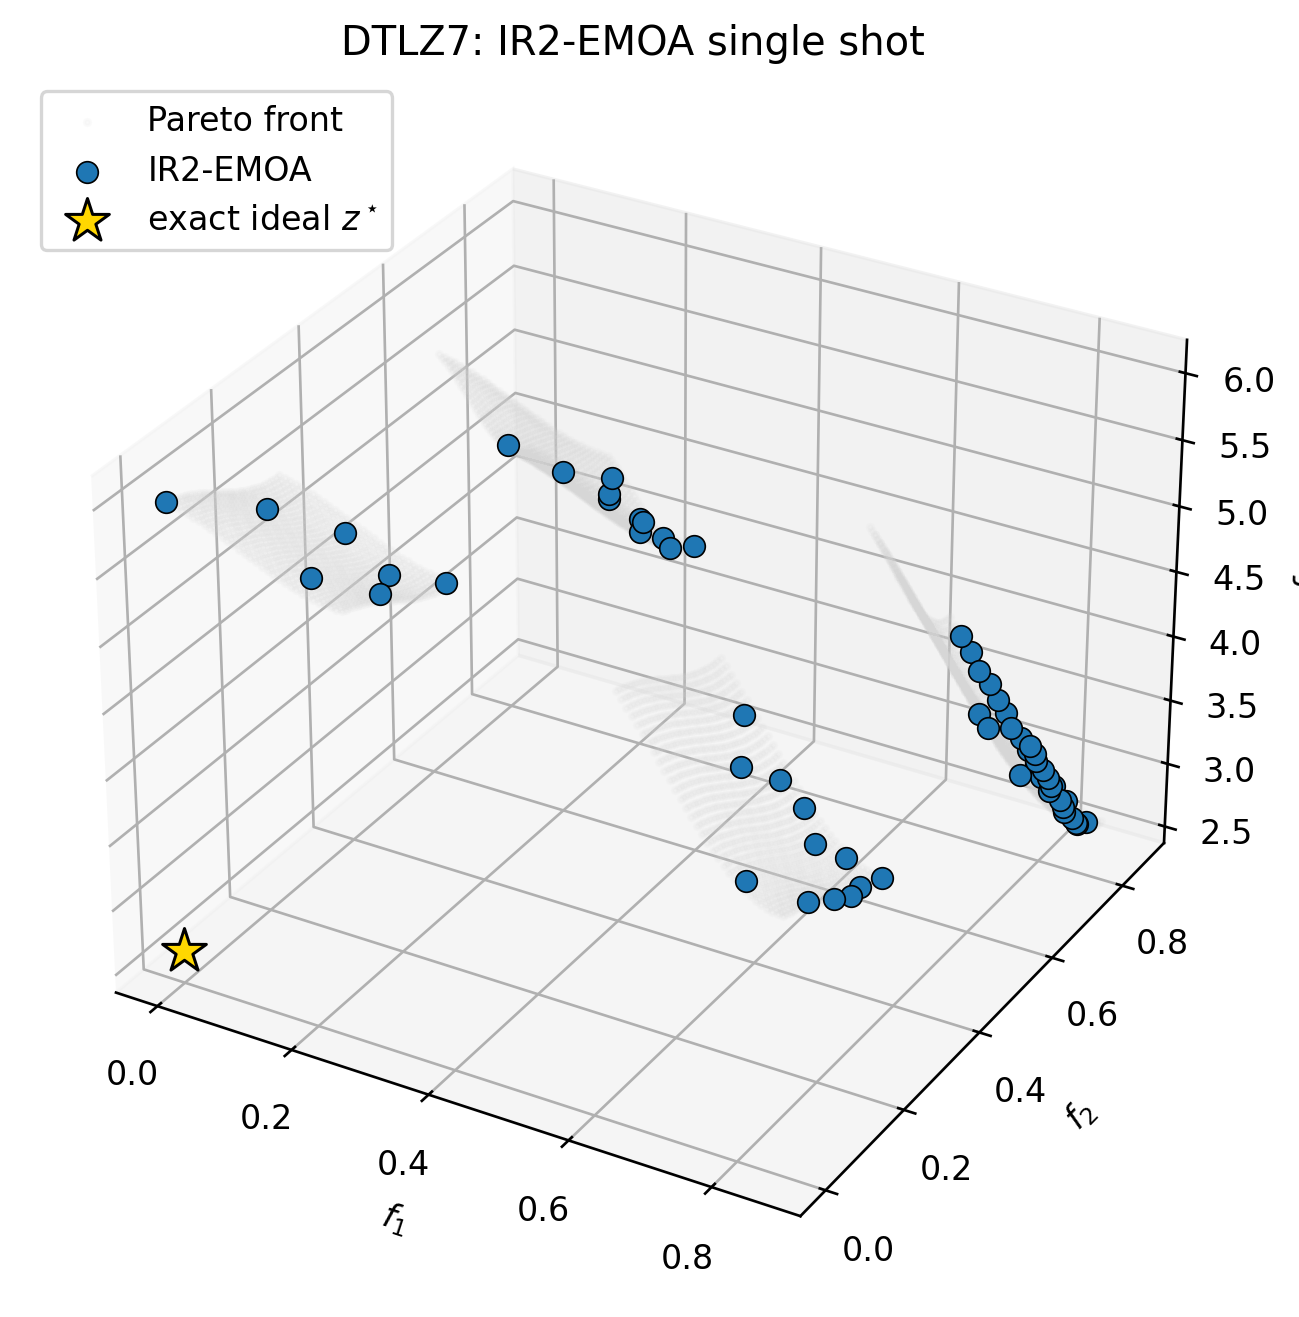
\includegraphics[width=0.45\linewidth]{single_shot_dtlz7_3d_exact_ideal_60000evals.png}
\end{tabular}
\caption{Diagnostic gallery of exact-ideal single-shot IR2-EMOA runs. Light gray points show the sampled Pareto front, dark points the final approximation, and the star the exact ideal point.}
\label{fig:single-shot-gallery}
\end{figure}

\section{Discussion}
\label{sec:discussion}

The intended comparison is not ``Integral R2 versus every indicator.'' Rather, it evaluates two closely related steady-state indicator-based selection principles. SMS-EMOA uses a Pareto-compliant unary indicator referenced to a dystopian point; IR2-EMOA uses a Pareto-compliant unary indicator referenced to an ideal point. The contrast is therefore meaningful even if neither algorithm uniformly dominates the other across front geometries.

A second comparison concerns discretization. Finite-weight R2-EMOA approximates the distribution of Tchebycheff utilities with finitely many directions. Integral R2 removes that discretization and consequently avoids zero sensitivity caused solely by unsampled weight regions. This does not imply that finite-weight R2 is obsolete: finite weights remain useful when explicit preference directions are desired. The present paper instead studies the preference-neutral uniform integral and its use for general-purpose environmental selection.

The scope has two deliberate limitations. First, only two and three objectives are considered, because exact low-dimensional algorithms make steady-state deletion practical and because the paper is about the algorithmic consequences of exact Integral R2 rather than many-objective approximation. Second, the present formulation assumes an available fixed ideal/utopian point. Adaptive or uncertain reference information is outside the scope of this study.

\section{Conclusion}
\label{sec:conclusion}

We introduced Integral R2 EMOA (IR2-EMOA), a steady-state indicator-based EMOA that deliberately follows the $\mu+1\rightarrow\mu$ selection structure of SMS-EMOA but uses exact IR2 contribution in place of hypervolume contribution. Integral R2 is a unary Pareto-compliant indicator obtained by integrating weighted Tchebycheff losses over a continuous weight simplex and is naturally referenced to an ideal/utopian point. In two objectives, IR2-EMOA directly uses the contribution method already available from R2 v2. In three objectives, perspective mapping transforms IR2 contributions into weighted exclusive orthogonal-box measures, enabling the reuse of efficient low-dimensional contribution sweeps with a different box integral. The resulting method provides a focused alternative to both hypervolume-based SMS-EMOA and finite-weight R2-EMOA for two- and three-objective optimization.

In the ten-run benchmark, IR2-EMOA attains the smallest median Integral R2 on five of the six problems, while SMS-EMOA attains the largest median hypervolume on all six. The $\Delta_p$ results are more mixed, with the best median values distributed across the three selection mechanisms. These results support the intended interpretation of IR2-EMOA as a distinct indicator-based selection principle with its own distributional bias, rather than as a uniformly superior replacement for hypervolume- or finite-weight R2-based selection.

\subsubsection*{Open-source implementations and support material}
The perspective-mapping implementation used as the computational basis for Integral R2 is publicly available at
\url{https://github.com/emmerichmtm/IntegralR2ByPerspectiveMapping}.
The supporting three-objective IR2 contribution calculator based on perspective mapping, hypervolume-analogue box decomposition, and dimension sweep is available at
\url{https://github.com/emmerichmtm/IntegralR2ContributionCalculator}.
The IR2-EMOA implementation and the scripts accompanying this paper are available at
\url{https://github.com/emmerichmtm/Integral-R2-EMOA}.
The source package accompanying the paper additionally contains the benchmark scripts, seeds, diagnostic gallery data, and the $10{,}000$-point Pareto reference sets used for Integral R2, HV, and $\Delta_p$ assessment.

% Bibliography included directly for a single-file submission source.
\begin{thebibliography}{12}
\providecommand{\url}[1]{\texttt{#1}}
\providecommand{\urlprefix}{URL }
\providecommand{\doi}[1]{https://doi.org/#1}

\bibitem{BeumeNaujoksEmmerich2007}
Beume, N., Naujoks, B., Emmerich, M.T.M.: {SMS-EMOA}: Multiobjective selection
  based on dominated hypervolume. European Journal of Operational Research
  \textbf{181}(3),  1653--1669 (2007). \doi{10.1016/j.ejor.2006.08.008}

\bibitem{BrockhoffWagnerTrautmann2012}
Brockhoff, D., Wagner, T., Trautmann, H.: On the properties of the {R2}
  indicator. Proceedings of the Genetic and Evolutionary Computation Conference
  (GECCO) pp. 465--472 (2012)

\bibitem{DebThieleLaumannsZitzler2002}
Deb, K., Thiele, L., Laumanns, M., Zitzler, E.: Scalable multi-objective
  optimization test problems. In: Proceedings of the 2002 Congress on
  Evolutionary Computation. vol.~1, pp. 825--830. IEEE (2002)

\bibitem{Emmerich2026Subset2D}
Emmerich, M.T.M.: Exact and fast subset selection algorithms for the
  bi-objective integral {R2} indicator. arXiv preprint arXiv:2606.23365 (2026)

\bibitem{Emmerich2026Subset3D}
Emmerich, M.T.M.: Three-objective integral {R2} subset selection: {NP}-hardness
  and submodular approximation. arXiv preprint arXiv:2606.26591 (2026)

\bibitem{Emmerich2026Perspective}
Emmerich, M.T.M.: Computing the integral {R2} indicator by perspective mapping
  and box decomposition. arXiv preprint arXiv:2606.30530  (2026)

\bibitem{Emmerich2026Preference}
Emmerich, M.T.M.: Preference-shaped expected hypervolume and {R2} improvement:
  Exact computation and monotonicity. arXiv preprint arXiv:2605.28746  (2026)

\bibitem{EmmerichFonseca2011}
Emmerich, M.T.M., Fonseca, C.M.: Computing hypervolume contributions in low
  dimensions: Asymptotically optimal algorithm and complexity results. In:
  Evolutionary Multi-Criterion Optimization (EMO 2011). Lecture Notes in
  Computer Science, vol.~6576, pp. 121--135. Springer (2011).
  \doi{10.1007/978-3-642-19893-9_9}

\bibitem{JaszkiewiczZielniewicz2025}
Jaszkiewicz, A., Zielniewicz, P.: Exact calculation and properties of the {R2}
  multiobjective quality indicator. IEEE Transactions on Evolutionary
  Computation  \textbf{29}(4),  1227--1238 (2025).
  \doi{10.1109/TEVC.2024.3440571}

\bibitem{PhanSuzuki2013}
Phan, D.H., Suzuki, J.: {R2-IBEA}: {R2} indicator based evolutionary algorithm
  for multiobjective optimization. In: 2013 IEEE Congress on Evolutionary
  Computation (CEC). pp. 1836--1845. IEEE (2013).
  \doi{10.1109/CEC.2013.6557783}

\bibitem{SchaepermeierKerschke2025}
Sch{\"a}permeier, L., Kerschke, P.: {R2 v2}: The pareto-compliant {R2}
  indicator for better benchmarking in bi-objective optimization. Evolutionary
  Computation  (2025). \doi{10.1162/EVCO.a.366}, also available as
  arXiv:2407.01504

\bibitem{SchuetzeEtAl2012}
Sch{\"u}tze, O., Esquivel, X., Lara, A., Coello, C.A.C.: Using the averaged
  hausdorff distance as a performance measure in evolutionary multiobjective
  optimization. IEEE Transactions on Evolutionary Computation  \textbf{16}(4),
  504--522 (2012). \doi{10.1109/TEVC.2011.2161872}

\bibitem{TrautmannWagnerBrockhoff2013}
Trautmann, H., Wagner, T., Brockhoff, D.: {R2-EMOA}: Focused multiobjective
  search using {R2}-indicator-based selection. In: Learning and Intelligent
  Optimization (LION 7). Lecture Notes in Computer Science, vol.~7997, pp.
  70--74. Springer (2013). \doi{10.1007/978-3-642-44973-4_8}

\end{thebibliography}

\end{document}
